\chapter{Results}

In this chapter we present our investigations in numerical simulations using methods from \textbf{Simulations} chapter, and measurements from oscillatory experiments introduced in \textbf{Experimental Approach} chapter.

In the first part of this chapter, we analyse the functionality of new codebase. We made several tests on energy conservation, precision of numerical methods and stability, to ensure that simulation is reliable and stable for further development.

In the second part, we present our drag force measurements by using the oscillators. We start with the two-fluid regime (temperature above $T > 1.3 \unit{K}$) and connect these results with those from ballistic regime ((temperature below $T < 0.6 \unit{K}$)).

\section{Simulation experiments}
% \begin{itemize}
% 	\item does num segments affect the initial ring velocity?
% 	\item does energy (and velocity) changes if Quantum=False?
% 	\item for a given R and euler method, what is the life of stability for various num segments
% 	\item when is it good to resegment?
% 	\item which config leads to the death of the ring for various R
% 	\item measure death time and distance for various R
%
% \end{itemize}
%
% \section{Vortex ring}
% \begin{itemize}
% 	\item compare rings with various radii
% 	\item theoretical vs simulation velocity / range
% 	\item stability tests
% 	\item initialisation
% 	\item movement, decreasing radius
% 	\item comparison with theory
% \end{itemize}

All presented measurements and results were done in order to setup the \texttt{config} file and thus to recommend the best simulation parameters for future investigations. We performed tests with physical motivation and also tests focused on precision and stability. With presented findings, there should be ensured the reliability and stability of any further high-scale simulation.

\newpage

%%%%%%%%%%%%%%%%%%%%%%%%%%%%%%%%%%%%%%%%%%%%%%%%%%%%%%%%%%%%%%%%%%%%%%%%%%%%%%%%%%%%%%%%%%%%%%%%%%%%%%%%%%%%%%%%%%%%%%%%%%%%%%%%%%%%%%%%%%%%%%%%%%%%%%%%%%%%

\subsection*{Zero-temperature test}

In case of zero temperature $T=0\unit{K}$, there should be no \textit{normal component} in superfluid He-II and therefore also no mutual friction. In such case, velocity and energy of vortex ring is conserved due to the lack of energy dissipation processes.

We plotted in \textbf{Figure \ref{Tzero}} the ring velocity $\vert \vec{v}_{\text{ring}} \vert $ and energy $E_{\text{ring}}$ evoluting in time, for the case of temperature $T=0$ (pure superfluid, no normal component) and $T=1.5\unit{K}$ (considerable ratio of present normal and superfluid component).\\ We tested the mutual friction effect during 1000 time-steps (calling \textit{epochs}) with varying $\text{d}t$ according to (\ref{adaptive_dt}).

\begin{figure}[h]
	\centering
	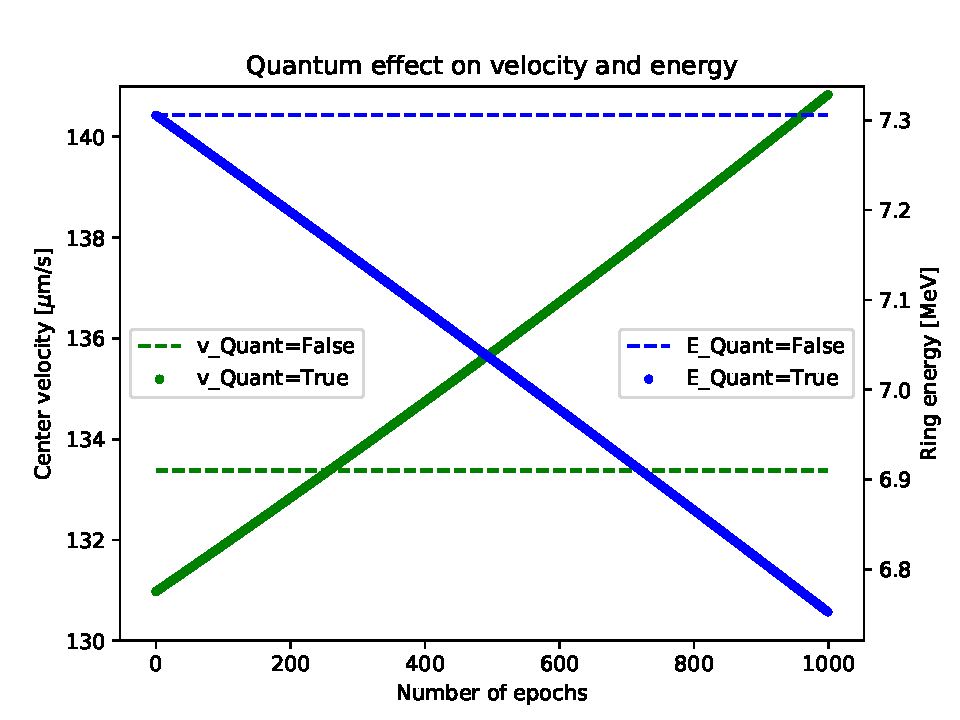
\includegraphics[width=0.8\textwidth]{graphics/results/Tzero}
	\caption{Evolution of ring velocity and energy in time. \underline{Blue lines} - measured velocity data, \underline{Black lines} - measured energy data,
	\underline{Dashed lines} - the constant behaviour for temperature $T=0\unit{K}$, \underline{Full lines} - the dissipative process for temperature $T=1.5\text{K}$.\\
	On \texttt{x} axis, we plot the number of elapsed epochs (time steps) and on \texttt{y} axis the velocity of the ring center $\vert \vec{v}_{\text{ring}} \vert $ and ring energy $E_{\text{ring}}$.}
	\label{Tzero}
\end{figure}

As we see, at $T=0\unit{K}$ the velocity and energy is conserved even after 1000 epochs of simulation due to missing dissipation process (mutual friction). In case of $T=1.5\unit{K}$, energy is falling down as expected, whereas the velocity is increasing. This increase is physically well-explained by the fact that the radius is decreasing with time due to the non-dissipative term of mutual friction. Also, the thoretical formula (\ref{ring-velocity})

%%%%%%%%%%%%%%%%%%%%%%%%%%%%%%%%%%%%%%%%%%%%%%%%%%%%%%%%%%%%%%%%%%%%%%%%%%%%%%

\subsection*{Velocity precision test}

Our first velocity test compares the various approaches how can the ring velocity $\vert \vec{v}_c \vert $ be calculated. Here, we recognize between four approaches, based on its theoretical motivation, computational complexity and precision:
\begin{itemize}
	\item LIA (\ref{LIA}): motivated \cite{barenghi}, computationally cheap, not precise
	\item LIA + BIOT (\ref{LIA} + \ref{BIOT}): motivated \cite{barenghi}, but computationally expensive
	\item updated LIA (\ref{LIAnew}): not well motivated \cite{samuels}, but computationally cheap and precise
	\item Theoretical (\ref{ring-velocity}): well motivated \cite{roberts} and most precise
\end{itemize}

\begin{figure}[h]
	\centering
	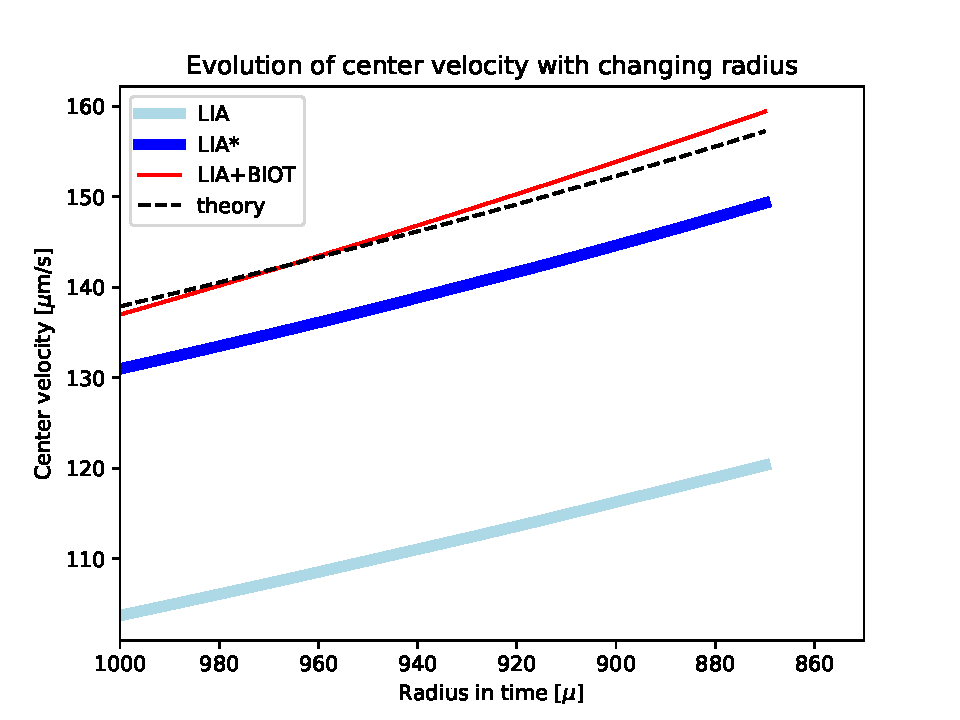
\includegraphics[width=0.8\textwidth]{graphics/results/vels_radius}
	\caption{Comparison of all implemented velocity approaches (\underline{full lines}) with the theoretical one (\underline{black dashed line}) according to (\ref{ring-velocity}), with decreasing radius in time.\\
	On \texttt{x} axis, we plot the number of elapsed epochs (time steps) and on \texttt{y} axis the ring velocity $\vert \vec{v}_{\text{ring}} \vert$.}
	\label{vels-radius}
\end{figure}

The theoretical values for velocity from (\ref{ring-velocity}) is taken as a baseline that other velocity calculations are compared with. All velocites were
measured and evoluted over a few thousands epochs (time steps), during which the radius was dissipatively decreasing, as is sketched in \textbf{Figure \ref{vels-radius}}.

We see that the theoretically most precise (LIA + BIOT) approach grows a bit faster than it should according to theory. This inconsistence is caused by bad resolution parameter, which was set at $\delta \approx 70 \mu \unit{m}$\\
Therefore, for all further measurements we used the updated LIA velocity (LIA*) approach due to its time-scale consistancy and computational speed.

%%%%%%%%%%%%%%%%%%%%%%%%%%%%%%%%%%%%%%%%%%%%%%%%%%%%%%%%%%%%%%%%%%%%%%%%%%%%%%

\subsection*{Velocity convergence test}

Next, we investigated the magnitude of the ring velocity $\vert \vec{v}_{\text{ring}} \vert$ for various resolutions $\delta \in \langle 50, 200 \rangle \mu\text{m}$, immediately after initialisation and then after 100 epochs. Ring radius was always set at $R=1000\mu\text{m}$ (this is usual working radius \cite{tsubota} \cite{FDclosed}), so the number of discretisation points along the vortex was given by $R$ and $\delta$ as $N \approx 2\pi R/ \delta \in \langle 30,120 \rangle$.

\begin{figure}[h]
	\centering
	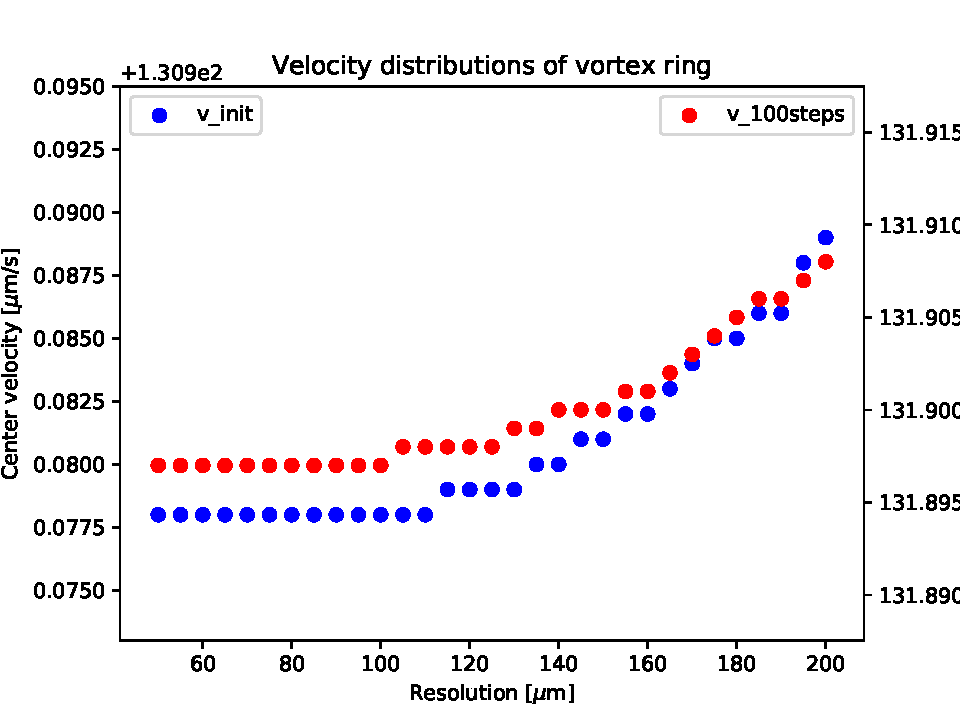
\includegraphics[width=0.8\textwidth]{graphics/results/vels_convergence}
	\caption{The distribution of ring velocity values $\vert \vec{v}_{\text{ring}} \vert$ for a range of resolution paramters $\delta$ in two situations. \underline{Blue dots} - Velocity values immediately after initialisation, \underline{Red dots} - velcotiy values after 100 time-steps.\\
	On \texttt{x} axis, we plot the resolutions $\delta$ of vortex segments and on \texttt{y} axis the ring velocity $\vert \vec{v}_{\text{ring}} \vert$.}
	\label{vels-converg}
\end{figure}

We see in \textbf{Figure \ref{vels-converg}} the expected convergent behaviour of both measured velocities in an area of good resolutions (small values of $\delta$). It seems that below $ \delta < 100 \mu\text{m}$  (corresponding to $\approx 60$ segments along the ring of radius $R=1000 \mu \unit{m}$) the velocites perform enough convergent behaviour, which provides the upper boundary for a \textit{good-chosen} resolution.

Even if it is intuitive that good resolutions (small $\delta$-s) lead to more precise velocities, the high number of vortex segments $N \propto 1/\delta$ worsens the stability of simulation in time. The reason behind this effect is the assumption of \textit{RK4} stepping method that functions, which \textit{RK4} is approximating, are smooth. With higher number of segmnets, there is higher chance for the ring to be non-smooth, which leads to an exponential errors in \textit{RK4} algorithm.

Therefore, we propose also a lower boundary $\delta_{\text{min}}$, ensuring the stability, in a following test in next subsection.

%%%%%%%%%%%%%%%%%%%%%%%%%%%%%%%%%%%%%%%%%%%%%%%%%%%%%%%%%%%%%%%%%%%%%%%%%%%%%%

\subsection*{Stability test}

Stability of simulation in time was measured for a range of resolutions $\delta \in \langle 10, 100 \rangle \mu\text{m}$ and three values of vortex radius $R \in \{500, 1000, 2000\} \mu\text{m}$ using \textit{Euler} and \textit{RK4} stepping method. In all cases, the stability is measured by the maximal number of elapsed epochs, till the simulation was forced to stop.
This enforcement was determined by the violation of length condition, as was described in \textbf{Real-time tests} subsection- the real vortex circumference $l = \sum_j \vert \vec{s}_j - \vec{s}_{j+1} \vert$ cannot deviate more than $1\%$ from the geometrical value $2\pi R$, where $R$ is the measured radius in current state.

\begin{figure}[h]
	\centering
	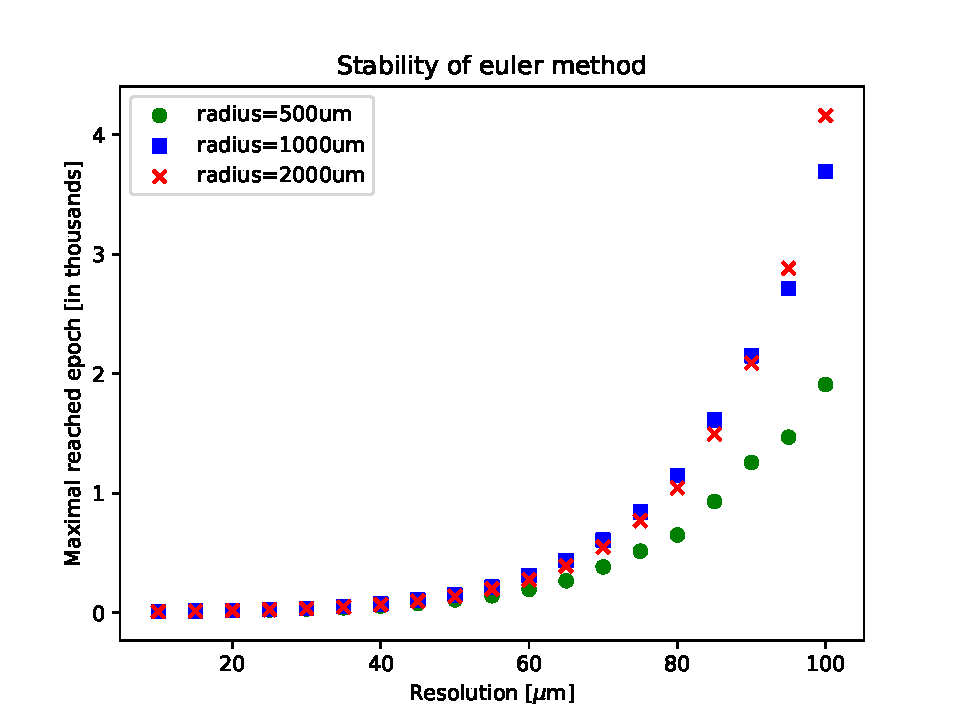
\includegraphics[width=0.8\textwidth]{graphics/results/stability-euler}
	\caption{Plot of maximal elapsed epoch (time step) of simulation with a given resolution $\delta$, radius $R$ and \textit{Euler} stepping method, till the simulation was forced to stop by violating the length condition.}
	\label{stab-euler}
\end{figure}


From the plot in \textbf{Figure \ref{stab-euler}}, the \textit{Euler} method seems to be unstable for whatever resolution $\delta \in \langle 10, 100 \rangle \mu\text{m}$. Such behaviour was expected and simulated only as an example of really wrongly chosen stepping method.

The next experiment was conducted with \textit{RK4} method, a much stable method comparing with the \textit{Euler} one, but also suffering from strong assumptions (smoothness of evoluting function). Nevertheless, the plot of maximal reached epoch performed is much more stable:

\begin{figure}[h]
	\centering
	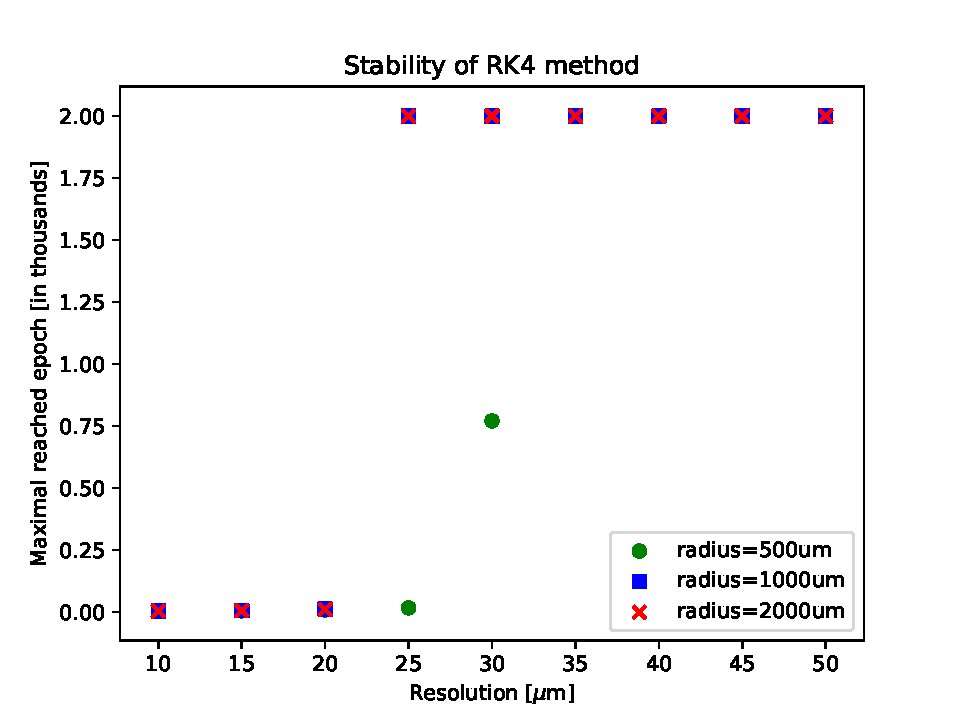
\includegraphics[width=0.8\textwidth]{graphics/results/stability-RK4}
	\caption{Plot of maximal elapsed epoch (time step) of simulation with a given resolution $\delta$, radius $R$ and \textit{RK4} stepping method, till the simulation was forced to stop by violating the length condition. A threshold is set on $2000$ epochs.}
\end{figure}

The plot in \textbf{Figure 14} suggests the minimal resolution to be at least $\delta >30\mu\text{m}$. This boundary estimate is still quite conservative, since the radius of vortex is decreasing in time and resegmentation processes will happen.
Resegmantation process heavily help to the stability of simulation since the deletion a of some segments works as a \textit{smoothing effect} which supports the \textit{RK4} method to be stable.

\newpage

%%%%%%%%%%%%%%%%%%%%%%%%%%%%%%%%%%%%%%%%%%%%%%%%%%%%%%%%%%%%%%%%%%%%%%%%%%%%%%
